\documentclass[11pt]{report}
\usepackage[utf8]{inputenc}
\usepackage[danish]{babel}
\usepackage [T1]{fontenc}
\usepackage[margin=2.5cm]{geometry}
\usepackage[hidelinks]{hyperref}
\usepackage{graphicx}
\graphicspath{{figures/}{Billeder/}}
\usepackage{listings}
\usepackage{color}
\usepackage{adjustbox}
\usepackage{tocloft}

\definecolor{bluekeywords}{rgb}{0.13,0.13,1}
\definecolor{greencomments}{rgb}{0,0.5,0}
\definecolor{turqusnumbers}{rgb}{0.17,0.57,0.69}
\definecolor{redstrings}{rgb}{0.5,0,0}

\lstdefinelanguage{FSharp}
                {morekeywords={let, new, match, with, rec, open, module, namespace, type, of, member, and, for, in, do, begin, end, fun, function, try, mutable, if, then, else},
    keywordstyle=\color{bluekeywords},
    sensitive=false,
    morecomment=[l][\color{greencomments}]{///},
    morecomment=[l][\color{greencomments}]{//},
    morecomment=[s][\color{greencomments}]{{(*}{*)}},
    morestring=[b]",
    stringstyle=\color{redstrings}
    }
\usepackage{amsmath}
\title{Cupcake}
\author{
    Asger Hermind Sørensen\\
    Department\\
    school\\
    email@edu
  \and
    William Sehested Huusfeldt\\
    Department\\
    school\\
    email@edu
  \and
    Andreas Vikke\\
    Department\\
    school\\
    email@edu
  \and
    Martin Eli Frederiksen\\
    Department\\
    school\\
    email@edu
}

\date{\today}

\begin{document}
\maketitle

\renewcommand{\cftchapleader}{\cftdotfill{\cftdotsep}}
\tableofcontents
\newpage

\chapter*{1. Indledning}
\addcontentsline{toc}{chapter}{1. Indledning}
Dummy text
\begin{center}
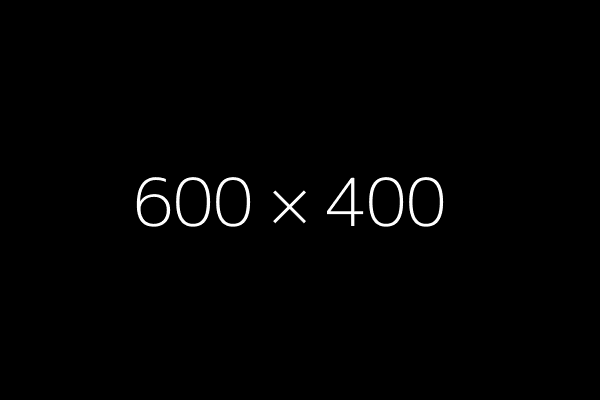
\includegraphics[width=15cm]{fff.png}
\end{center}

\newpage

\chapter*{2. Baggrund}
\addcontentsline{toc}{chapter}{2. Baggrund}
Dummy text
\section*{2.1. Virksomheden}
\addcontentsline{toc}{section}{2.1. Virksomheden}
Dummy text
\section*{2.2. Virksomhedens krav}
\addcontentsline{toc}{section}{2.2. Virksomhedens krav}
Dummy text
\section*{2.3. Virksomhedens vision}
\addcontentsline{toc}{section}{2.3. Virksomhedens vision}
Dummy text

\newpage

\chapter*{3. Sprog og programmer}
\addcontentsline{toc}{chapter}{3. Sprog og programmer}
Dummy text

\newpage

\chapter*{4. ER Diagram}
\addcontentsline{toc}{chapter}{4. Baggrund}
Dummy text

\newpage

\chapter*{5. Navigationsdiagram}
\addcontentsline{toc}{chapter}{5. Navigationsdiagram}
Dummy text

\newpage

\chapter*{6. Sekvens diagrammer}
\addcontentsline{toc}{chapter}{6. Sekvens diagrammer}
Dummy text

\newpage

\chapter*{7. Struktur}
\addcontentsline{toc}{chapter}{7. Struktur}
Dummy text

\newpage

\chapter*{8. Særlige forhold}
\addcontentsline{toc}{chapter}{8. Særlige forhold}
Dummy text

\newpage

\chapter*{9. Manglende implementer}
\addcontentsline{toc}{chapter}{9. Manglende implementer}
Dummy text

\newpage

\chapter*{10. Links og referencer}
\addcontentsline{toc}{chapter}{10. Links og referencer}
\begin{itemize}
  \item CupCake Webshop: \url{http://andreasvikke.dk/CupCake/}
  \item GitHub: \url{https://github.com/Krigermus/CupCake/}
  \item JavaDoc: \url{http://andreasvikke.dk/CupCake-javadoc/}
\end{itemize}

 \newpage

\end{document}

